
%(BEGIN_QUESTION)
% Copyright 2011, Tony R. Kuphaldt, released under the Creative Commons Attribution License (v 1.0)
% This means you may do almost anything with this work of mine, so long as you give me proper credit

Calculate the following parameters in this three-phase (balanced) AC power system:

$$\includegraphics[width=15.5cm]{i03597x01.eps}$$

\begin{itemize}
\item{} $V_{line}$ (generator) = 
\vskip 10pt
\item{} $I_{line}$ (generator) = 
\vskip 10pt
\item{} $V_{line}$ (load) = 
\vskip 10pt
\item{} $I_{line}$ (load) = 
\vskip 10pt
\item{} $P_{total}$ = 
\end{itemize}

\vfil 

\underbar{file i03597}
\eject
%(END_QUESTION)





%(BEGIN_ANSWER)

This is a graded question -- no answers or hints given!

%(END_ANSWER)





%(BEGIN_NOTES)

Important concepts to keep in mind when analyzing three-phase networks is that of {\it series} and {\it parallel} connections: series-connected components must always share the same amount of current, while parallel-connected components must always share the same amount of voltage.  This is why line current and phase current are identical in wye networks: because each phase element is directly in series with each line conductor.  This is why line voltage and phase voltage are identical in delta networks: because each phase element is directly in parallel with a pair of line conductors.

\vskip 10pt

\begin{itemize}
\item{} $V_{line}$ (generator) = 4160.4 volts
\item{} $I_{line}$ (generator) = 0.045 amps
\item{} $V_{line}$ (load) = 360.3 volts
\item{} $I_{line}$ (load) = 0.52 amps
\item{} $P_{total}$ = 324.5 watts
\end{itemize}

Perhaps the most important insight into solving this problem is to realize that the transformer bank is connected in a Delta-Wye configuration (primary Delta and secondary Wye).  Thus, each transformer primary sees generator line voltage, while each transformer secondary sees load phase voltage.

%INDEX% Electronics review: 3-phase voltage/current/power calculation

%(END_NOTES)


